\section{Behavioral Coordination Approaches}
\todo{To split the figure}

In this section, we focus on approaches in which the emerging system behavior is obtained by specifying a \emph{model of coordination}. Such a model defines how behavioral models interact. We begin this section by approaches that enables a system designer to specify the coordination between models, \ie \emph{Coordination Languages} (At bottom of Figure~\ref{fig:coordapp}). We continue this section by presenting approaches that specify the coordination between languages in order to automate the coordination between models, \ie~\emph{Coordination Pattern Approaches} (At top of Figure~\ref{fig:coordapp}).

\begin{figure}
      \begin{center}
         			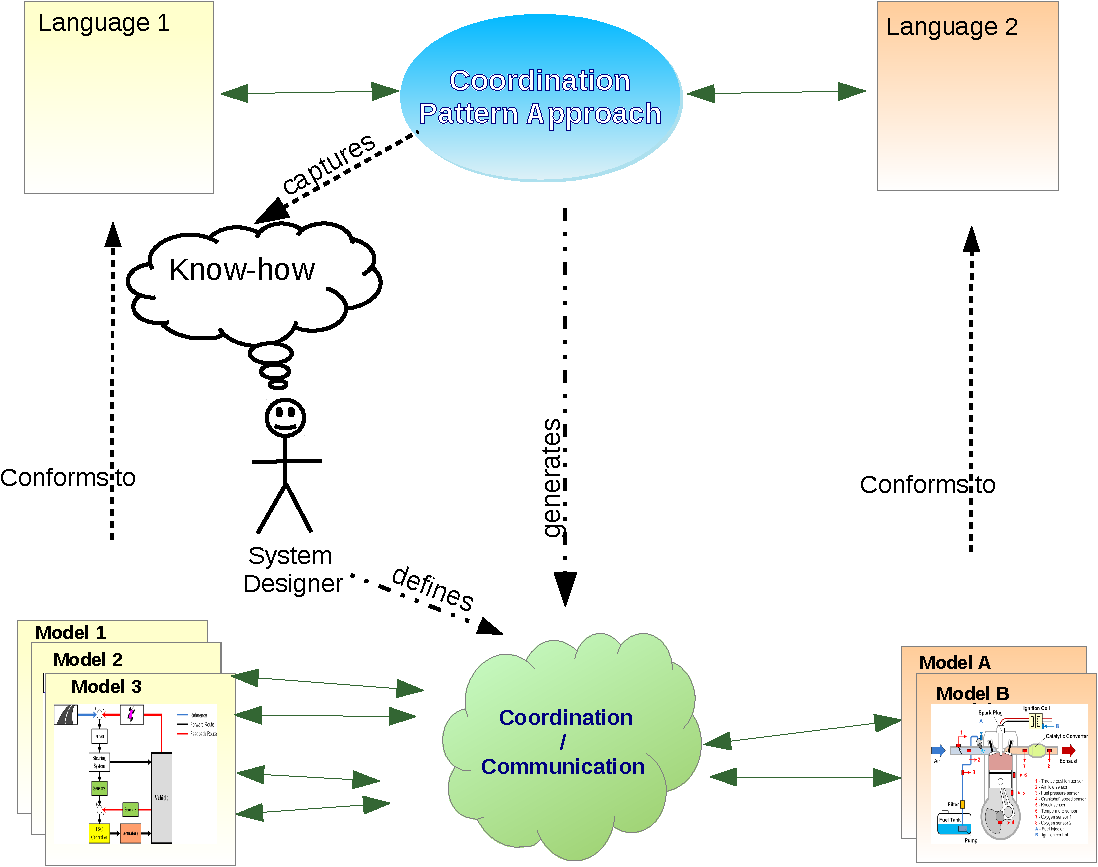
\includegraphics[width=0.6\columnwidth]{background/figs/coordpatterapp}
         			\caption{Overview of a Coordination Approaches}
         			\label{fig:coordapp}
        \end{center}
\end{figure}


\subsection{Coordination of Behavioral Models}
Coordination of Models approaches propose to specify the coordination at the model level. To do so, a system designer can use either a \emph{Coordination Language}~\cite{coordmodels} or an \emph{Architecture Description Language}~\cite{frameadlsbib}. In the following, we overview these approaches. 
			 
Coordination language approaches tackle the development of heterogeneous system by separating the computation concerns from the coordination concerns. They provide a dedicated language (\eg Esper~\cite{esperbib}, Linda~\cite{lindabib}, Manifold~\cite{manifoldbib}) for the specification of the coordination between behavioral models. A system designer defines one or more coordination model(s) to specify how the system models interact. According to \cite{coordsignibib}, ``\textit{Coordination is the process of building programs by gluing together active pieces}''. In~\cite{wegnercoorbib}, authors highlighted that the design of coordination languages must address the following issues: identification of the entities to coordinate, architecture style of the coordination and protocols/rules of coordination.

%More recently, BIP~\cite{bipbib} specifies the coordination or \emph{interactions} between \emph{components} by using \emph{connectors}. The approach provides a minimalist but expressive and formal algebra to specify the coordination between different automaton thus allowing the user to check properties like dead-lock freedom. Similarly, Metro2~\cite{metro2bib} relies on connectors and ports. However, while Metro2 enables to coordinate heterogeneous components, in BIP the components can only encapsulates automaton models. \emph{CyPhyML}~\cite{semanicbackplane} is a language aimed at integrating models that can conform to heterogeneous modeling languages, \eg SySML, AADL. As authors state, it is an \emph{Integrated Models Language}. In this approach, the semantics of modeling languages is abstracted by using a semantic interface which contains the essential concepts for cross-domain integration. By using semantic translators, models are transformed into CyPhy model integration space according to their semantic interface~\cite{semanicbackplane}. Then, CyPhy is used to specify the integration between models. The specification is written in FORMULA thus providing verification and analysis of the integrated system. In CyPhy, the coordination is specified between particular models, in this sense, CyPhy remains a coordination language.
			 
In parallel, \emph{software architecture} research field dealt with the growing complexity of software system by proposing languages (\ie ADLs~\cite{frameadlsbib, garlansoftarchbib}) to gain abstraction, structuring and reasoning capabilities(\eg Rapide~\cite{rapidebib}, Wright~\cite{wrightbib}, Unicon~\cite{uniconbib}). An ADL specifies a system in terms of components and interactions among those components. Such languages helped to:
\begin{itemize}
	\item Clarify structural and semantics difference between components and interactions.
	\item Reuse and compose architectural elements.
	\item Identify/enforce commonly used patterns (\eg architectural styles).
\end{itemize}

Depending on the ADL, a \emph{Component} can for instance be an encapsulation of some procedure, an encapsulation of an object file or a (formal) abstraction of its behavior. Most of the ADLs in the literature rely on well identified \emph{Component Interfaces} to externally characterize the components. The interfaces are used by \emph{Connector}s, whose behavior is specified by a \emph{glue}. The connectors can represent a large variety of interactions (\eg procedure call, event broadcast or database queries) and the glue can be of very different complexity ranging from the identity function to complex protocol specification. More recent work has been proposed in~\cite{bipbib,metro2bib}. In BIP~\cite{bipbib}, interactions between automatons are based on connectors. Similarly, MetroII~\cite{metro2bib} relies on connectors and ports between components. However, while Metro2 enables to coordinate heterogeneous components, in BIP the components can only encapsulate automaton models.   
			 			
Coordination languages and ADLs have common objectives~\cite{coordmodels}. They build/understand/analyse a system based on ``components'' (possibly written in different languages) and connectors (which include the specification of the interaction/coordination). Furthermore, they make a clear separation between two distinct activities in the development of a system: the specification of the different component of a system (\ie the computational aspects) and the assembly of these components (\ie the communication/coordination aspects). The first activity is usually performed by a software engineer and the second one is performed by a system designer. The system designer deals with the architecture-level communication that is expressed with complex protocols. To abstract away these protocols and make them reusable, ADLs propose connectors as types~\cite{frameadlsbib}. The main objective of that is to provide on the shelf connectors with domain specific interactions between components. 
			
Approaches like AADL~\cite{aadlbib} or Clara~\cite{clarabib} (to cite only two of them) proposed built-in connector and component types. These built-in types can either be part of the ADL or part of the architectural style (more details are provided in~\cite{taxonomyConnectors}). By providing built-in connector types, domain specific interaction can be reified. For instance, the Clara ADL is dedicated to real time systems, consequently it proposed built-in connector types like \emph{Rendez-vous}, \emph{Mutex} or \emph{Mailboxes}. This reification of coordination helps the coordination tasks by providing relevant domain specific connectors. It also limits what can appear in the interaction and is a step towards providing domain specific reasoning.
			
			
			\begin{figure}
				\begin{center}
					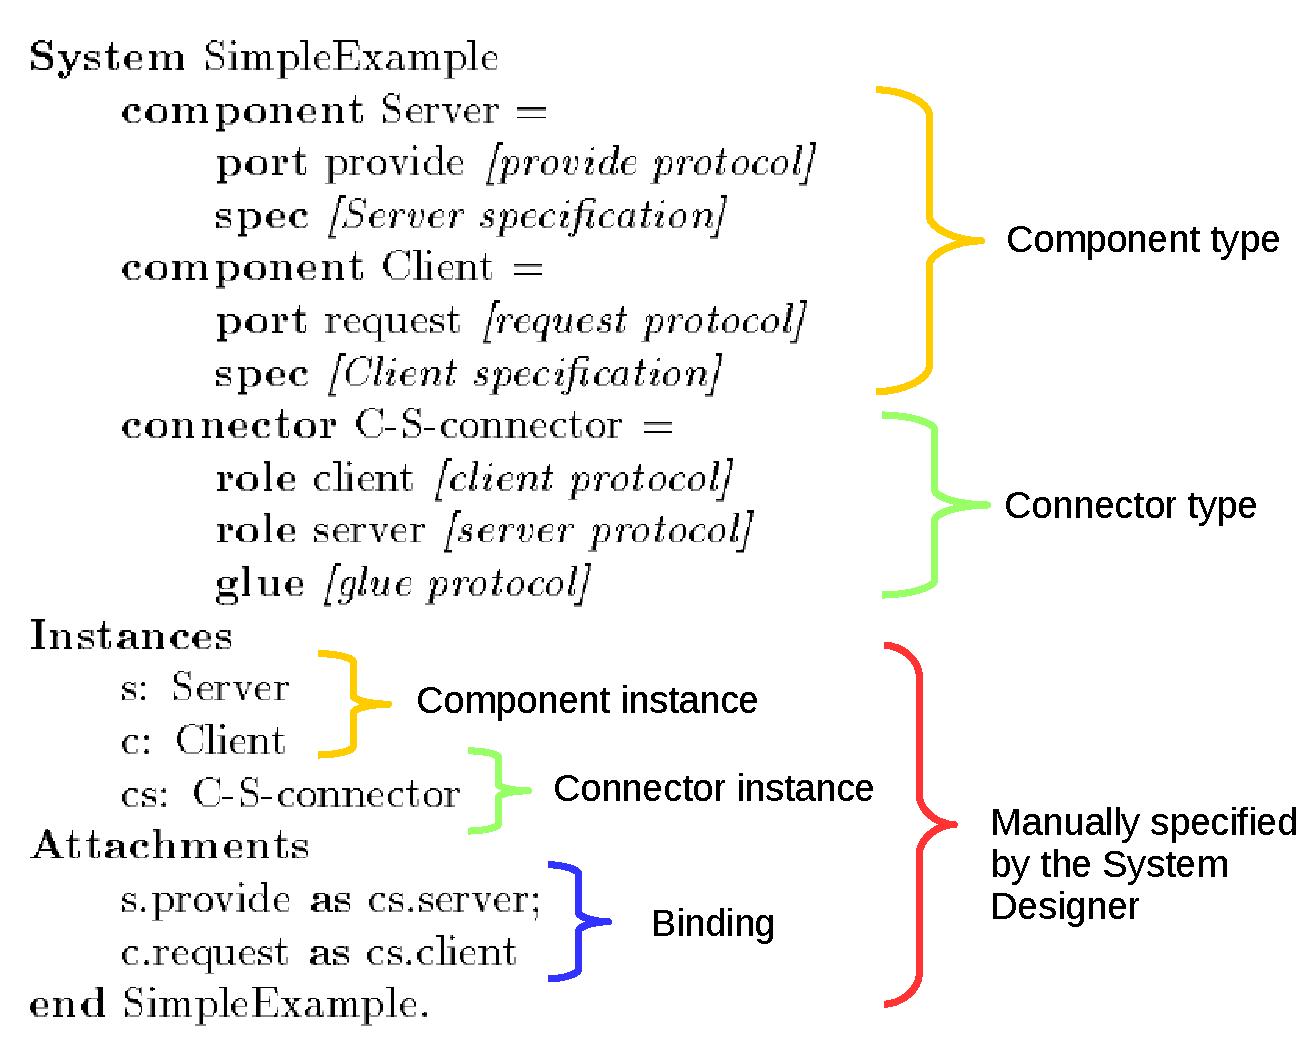
\includegraphics[width=0.5\columnwidth]{background/figs/wrightspec}
					\caption{Specification of a Client-Server system in Wright~\cite{wrightbib}}
					\label{fig:wrightspec}
				\end{center}
			\end{figure}
			
Other approaches go one step forward and introduce a notion of user defined type~\cite{uniconbib,wrightbib,reobib}. These ADLs can then be specialized to a specific domain by the creation of domain specific types. A connector type is usually defined by a set of roles and a glue specification. Roughly speaking, a role represents a formal parameter that is used by the specification of the glue. The glue specification specifies how the activities of the roles are coordinated. This glue can be specified more or less formally depending on the domain need. For instance, in Wright~\cite{wrightbib}, the glue is specified in a variant of CSP~\cite{csphoarebib} while in Reo it is specified by the composition of dedicated primitives~\cite{reobib}. The connector types are later on instantiated and the roles are bound to the actual interfaces of the instances of components. Figure~\ref{fig:wrightspec} shows a simple client-server system described in Wright~\cite{wrightbib}. The specification defines two component types named \emph{Client} and \emph{Server}, and one connector type named \emph{C-S-connector}. The C-S-connector has two roles (\emph{client} and \emph{server}) and a glue that describes how the activities of the client and server roles are coordinated. The section \emph{Instances} describes a particular configuration by instantiating the corresponding components and connectors. The example describes a system where there is a single server (\emph{s}), a single client (\emph{c}) and a single connector (\emph{cs}). Then, the section \emph{Attachments} defines which component ports are attached to the connector roles. This example illustrates how a system designer can define a set of domain specific connector types, and then, instantiate and bind the connector types as needed by its architecture. These connector types are qualified as pattern of interactions in \cite{wrightbib}. 
			
The major drawback of these approaches is that the instantiation and binding of connector types is done manually by the system designer. Returning to the example of Figure~\ref{fig:wrightspec}, for each server and client in the system, the system designer has to instantiate two components and one connector. Then, he has to bind the component ports with the connector roles. With the increasing number and heterogeneity of the components, this task can quickly becomes difficult and error prone. More recent approaches~\cite{dinatale,mascotbib,ptoleframebib,modhelxbib} identified that the instantiation and binding of connector types can be a systematic activity the system designer repeats many times and can consequently be defined as a pattern. Such a pattern is based on the know-how of the system designer and sometimes on naming or organizational conventions adopted by the models. Thus, they have captured the specification of such a behavioral coordination pattern into a tool to automate the instantiation and binding of connector types. They specify the coordination between heterogeneous languages rather than between particular models (see Figure~\ref{fig:coordapp}). Such specification is then applied on models to instantiate a set of connector types and bind their instances. We refer to these approaches as \emph{Coordination Pattern Approaches}.
         
\subsection{Coordination Pattern Approaches}

\todo{To define what a coordination pattern is}

\todo{To define what a coordination pattern approach is}

%	\item We define a \emph{coordination pattern} as a systematic way to coordinate the behavior of models, based on the knowledge of a system designer. A similar notion of coordination pattern is presented by Hardebolle et al.~\cite{hardebollethese} under the wording of \emph{interaction pattern}. 
%\item An interaction pattern is the formalization of the know-how and the systematic way to solve a coordination problem on heterogeneous languages.
%\item We define a \emph{coordination pattern approach} an approach that captures a coordination pattern thus leveraging on the know-how a system designer. 
Coordination pattern approaches (\eg MASCOT~\cite{mascotbib}, Ptolemy~\cite{ptoleframebib}, ModHel'X~\cite{modhelxbib}) go further than Coordination Languages and ADLs since:          
\begin{itemize}
   \item They capture the know-how of a system designer into a coordination pattern. 
   \item They specify the pattern between a set of languages by relying on information about theirs syntaxes and semantics. 
   \item They automate the coordination between behavioral models by relying on a pattern.
\end{itemize}     	     	
\begin{figure}
\begin{center}
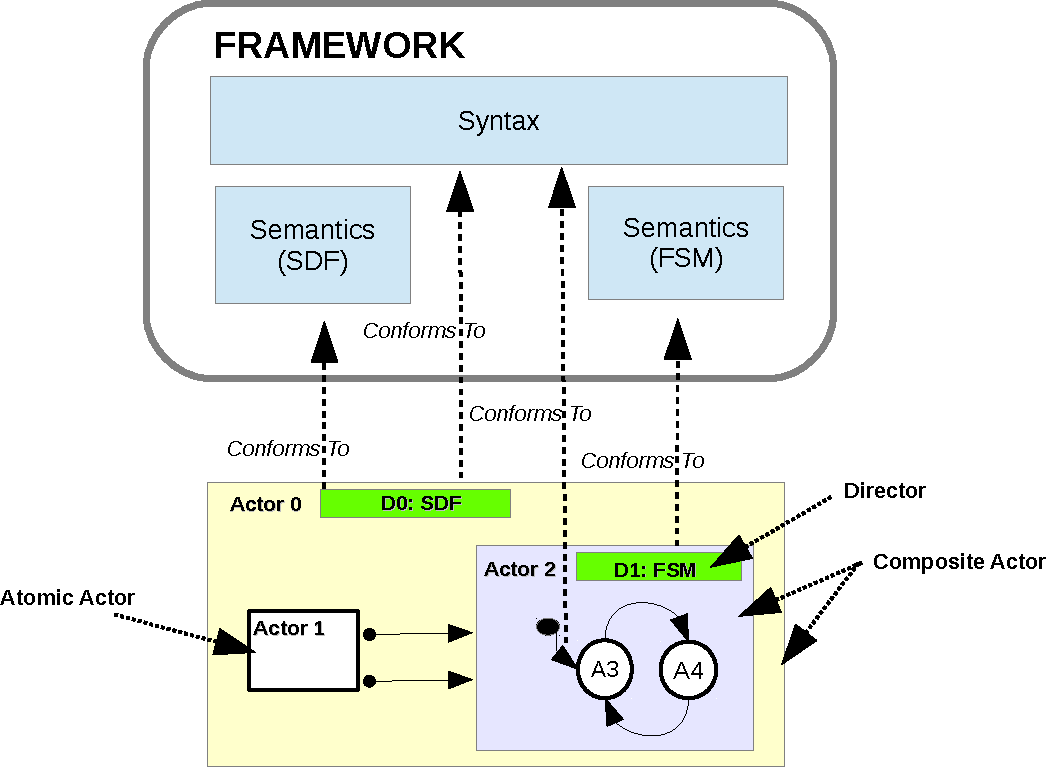
\includegraphics[width=0.7\textwidth]{background/figs/ptolemyfig}
\caption{High level view of Ptolemy~\cite{giraultbib}}
         			\label{fig:ptolemyfig}
         		\end{center}
\end{figure}
         	
Ptolemy~\cite{ptoleframebib} and ModHel'X~\cite{modhelxbib} are coordination frameworks that rely on a common syntax based on actors and a semantics given by Models of Computation (MoC). These approaches represent models as actors that can be atomic (\eg \emph{Actor 1} in Figure~\ref{fig:ptolemyfig}) or composite (\eg \emph{Actor 0} and \emph{Actor 2} in Figure~\ref{fig:ptolemyfig}), \ie made of internal actors. Each composite actor has associated a model of computation implemented as a \emph{Domain}. A domain defines the communication semantics and the execution order among internal actors. A domain is implemented by a \emph{Director}. For instance, in Figure~\ref{fig:ptolemyfig}, the \emph{Actor 0} has the director \emph{D0} that follows the semantics of SDF and the \emph{Actor 2} has the director \emph{D1} that follows the semantics of FSM. In this approach, actors, both atomic and composite, are executable. In a composite actor, the execution order of internal actors is controlled by a director. In the example of Figure~\ref{fig:ptolemyfig}, the director \emph{D0} controls the execution of the \emph{Actor 1} and \emph{Actor 2} and director \emph{D1} controls the execution of \emph{A3} and \emph{A4} whenever \emph{Actor 2} is executed. In this sense, the execution of composite actors is strictly hierarchical. The behavior of actors is represented by a generic interface that contains a set of methods, \eg fire(). The MoC implemented by the director of a composite actor specifies when the methods in the interface of internal actors are invoked. For instance, when a composite actor is fired, the director associated with the composite actor fires the actors of the contained model. Based on a fixed syntax and a generic interface, these approaches have achieved to capture a hierarchical coordination pattern into a framework. The framework provides a dedicated syntax to specified the pattern, \ie composite actors, and encodes the necessary glue between interfaces to coordinate their execution. 
         	

         	\begin{figure}
         		\begin{center}
         			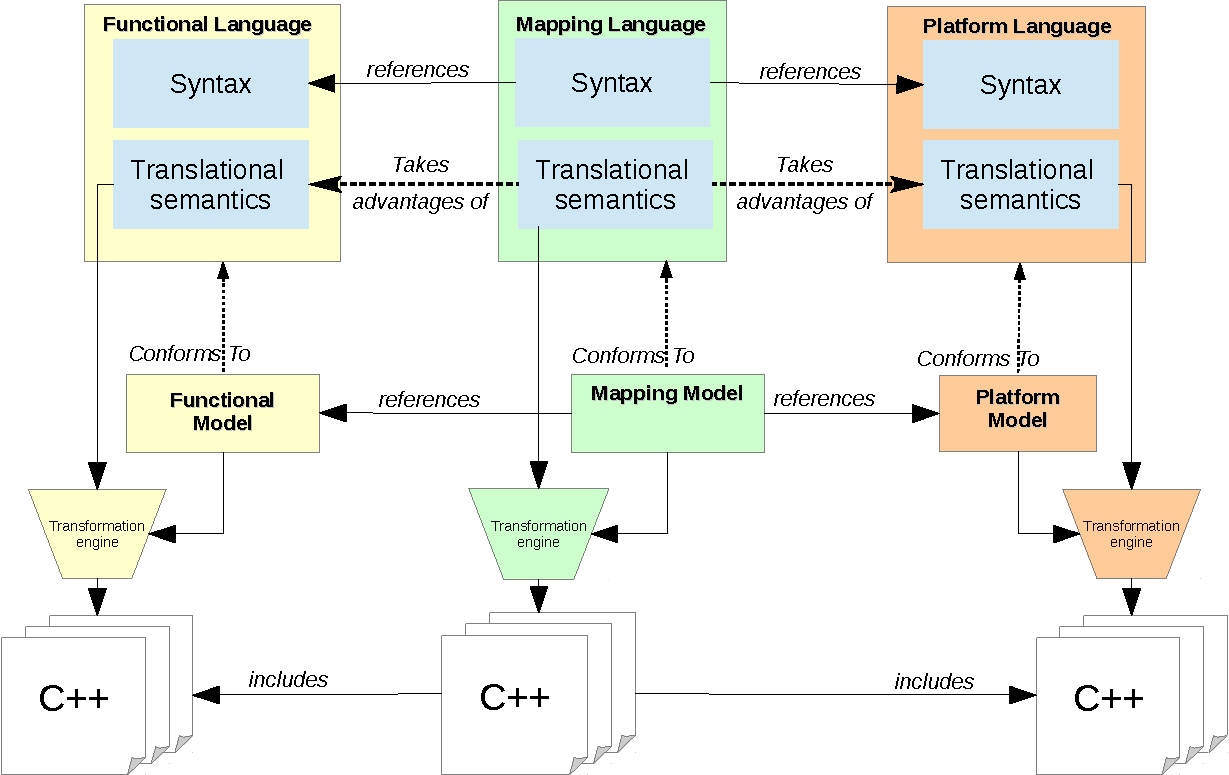
\includegraphics[width=0.7\textwidth]{background/figs/diNatale}
         			\caption{High Level view of the approach proposed by Di Natale et al. in~\cite{dinatale}}
         			\label{fig:diNatale}
         		\end{center}
         	\end{figure}

MASCOT~\cite{mascotbib} is a different approach focused on the integration of Matlab~\cite{matlabbib} and SDL~\cite{sdlbib}. Whereas SDL is a language suitable for control systems modeling, Matlab is better for modeling dataflow aspects of a system. However, these languages are very different, while SDL processes operate on events, represented by simple signals, Matlab processes operate on vectors, represented by vectorized signals. Thus, authors propose to automate the synchronization of control signals from SDL with data signals from Matlab. These signals can be either notification signals or message signals. Notification signals do not carry a value and are used to notify a process that an event has occurred. Message signals carry a value and are used to indicate a change of some variable or parameter. The approach deals with the integration of the timing and synchronization concepts from both languages by proposing two synchronization modes: head synchronization and tail synchronization. These mechanisms take advantages of the knowledge about the semantics of the languages. For instance, in the head synchronization, when a model in matlab receives a frame \emph{a1}, it immediately transforms \emph{a1} into \emph{b1} (dataflow network model). Any control signal from SDL that occurs during the transformation of \emph{a1} to \emph{b1} cannot influence its value. Then, the head synchronization mode ensures that the occurrence of the control signal is taken into account when the next frame is processed. In the tail synchronization, when a model in Matlab receives a control signal from SDL, the signal is collected until it cease to occur, then, it is translated to a vector and passed to the Matlab model. The modes of synchronization ensure the communication between Matlab and SDL. In addition, the approach gives a set of guidelines to aid the system designer to choose between the two synchronization proposed. Once the synchronization policy is defined, the approach enables the co-simulation of a SDL model and a Matlab model. The implementation is based on SDL wrappers. A process in the SDL specification that is specified in Matlab contains a wrapper that interfaces between the SDL simulator and the Matlab engine. A SDL wrapper is made of a set methods that enable the SDL engine to control the behavior of the data signals in Matlab. To do so, the approach relies on the name of signals in SDL specification to communicate with the signals in Matlab. The approach thus forces the system designer to follow a naming convention between signals in both domains. Although the current implementation partially automates the coordination of signals from both domains, the approach has identified and captured a coordination pattern between a control-flow language and a data-flow language by relying on some knowledge about its syntax and semantics.
         	
In~\cite{dinatale}, authors propose a dedicated language to map a functional model to a platform model (see Figure \ref{fig:diNatale}). Both the functional and the platform syntaxes were equipped with a translational semantics to C++ code. Then, based on the mapping model, the approach generates the code of the communication connectors between the code obtained from the functional and platform models. A first interesting aspect of this approach comes from the possibility, by creating a dedicated language, to reuse existing languages, and based on a mapping model to automatically generate the glue between the implementation of the models (in this case encoded in C++). By having a closer look at the approach, the mapping language syntax references syntactic elements from both the functional and the platform language. For instance, the $SWdeployment$ concept from the mapping model, reference the $Task$ concept from the functional model and the $CPU$ concept from the platform model. Also, the translational semantics of the mapping language takes advantages of some knowledges about the translational semantics of the other languages. For instance, for each subsystem, authors know that a class is generated with name \emph{SubsystemName}\texttt{ModelClass}. They also know that the class has a \texttt{step} operation for the runtime evaluation of the block outputs given the inputs and the state. In other words, authors have a partial but sufficient knowledge of the translational semantics of both the functional and the platform language. Finally, based on this knowledge, they encode in the translational semantics the glue to generate according to the actual mapping in the mapping model. The approach proposes a set of connectors that the system designer has to instantiate in the mapping model. In this sense, the approach is similar than the ADLs Clara, which proposes a set of built-in connectors. However, different than other ADLs, the approach proposes connectors that link concepts from different languages. In particular, these connectors capture some knowledge of a system designer that performs the mapping of a functional model to a platform model.
         	
\subsection{Discussion}

\todo{To avoid the summary}
Coordination languages approaches enable the system designer to define one or more models of coordination to specify how models interact. The main benefice of these approaches is that the global behavior is explicit and amenable for reasoning (for instance for Verification and Validation activities). However, if a similar problem occurs on different models, the system designer has to devise another coordination model. When applied to models, a coordination only captures the solution for one single problem and does not propose a commonly applicable solution for other coordination problems.
		
To capture once and for all the know-how of a system designer, coordination pattern approaches specify the coordination at the language level. Once a coordination pattern between a set of languages is captured, the models conforming to such languages can be coordinated automatically. Such approaches successfully capture the know-how of the integrator, however, they do so by embedding the coordination pattern inside a tool. As a result, the system designer cannot change the coordination specification without altering the core of the tool. However, for complex systems, the system designer may need to capture several coordination patterns and potentially combine them. This is highlighted in~\cite{giraultcompo} where authors use Ptolemy to capture three hierarchical coordination patterns between a finite state machine with Data flows, a Discrete event model and a Synchronous/Reactive model. Since each coordination pattern is applicable in different situations, authors argue that each one is useful. Thus, the system designer must be able to capture different coordination patterns since there is not necessarily a single \emph{valid} one. However, current coordination frameworks can only support such a variation by modifying the framework itself. Additionally, the coordination model is mixed with the functional model, which makes it very tricky to modify one without risking altering the other.
	
During the integration activity, the system designer must be able to capture different coordination patterns and their semantics must be explicit rather than being hidden inside a tool. To illustrate this, Gabor et al.~\cite{gaborpolyglot} show the semantic variations of Statecharts presented in different tools. Since each approach interprets differently the semantics of Statecharts, we obtain different behaviors depending on the approach. However, if the semantics is hidden inside the tool and is not made explicit, this can lead to misunderstandings and errors. Moreover, validation and verification activities are limited in current coordination frameworks since the coordination is encoded by using a general purpose language.
	